% Created 2025-05-17 Sat 17:04
% Intended LaTeX compiler: xelatex
\documentclass{article}


%%%%%%%% ICML 2025 EXAMPLE LATEX SUBMISSION FILE %%%%%%%%%%%%%%%%%
\usepackage[T1]{fontenc}
% Recommended, but optional, packages for figures and better typesetting:
\usepackage{microtype}
\usepackage{graphicx}
\usepackage{subfigure}
\usepackage{booktabs} % for professional tables

% hyperref makes hyperlinks in the resulting PDF.
% If your build breaks (sometimes temporarily if a hyperlink spans a page)
% please comment out the following usepackage line and replace
% \usepackage{icml2025} with \usepackage[nohyperref]{icml2025} above.
\usepackage{hyperref}


% Attempt to make hyperref and algorithmic work together better:
\newcommand{\theHalgorithm}{\arabic{algorithm}}

% Use the following line for the initial blind version submitted for review:
\usepackage[accepted]{style/icml2025}

% If accepted, instead use the following line for the camera-ready submission:
%% \usepackage[accepted]{style/icml2025}

% For theorems and such
\usepackage{amsmath}
\usepackage{amssymb}
\usepackage{mathtools}
\usepackage{amsthm}


% if you use cleveref..
\usepackage[capitalize,noabbrev]{cleveref}
%%%%%%%%%%%%%%%%%%%%%%%%%%%%%%%%
% THEOREMS
%%%%%%%%%%%%%%%%%%%%%%%%%%%%%%%%
\theoremstyle{plain}
\newtheorem{theorem}{Theorem}[section]
\newtheorem{proposition}[theorem]{Proposition}
\newtheorem{lemma}[theorem]{Lemma}
\newtheorem{corollary}[theorem]{Corollary}
\theoremstyle{definition}
\newtheorem{definition}[theorem]{Definition}
\newtheorem{assumption}[theorem]{Assumption}
\theoremstyle{remark}
\newtheorem{remark}[theorem]{Remark}

% Todonotes is useful during development; simply uncomment the next line
%    and comment out the line below the next line to turn off comments
%\usepackage[disable,textsize=tiny]{todonotes}
\usepackage[textsize=tiny]{todonotes}

% The \icmltitle you define below is probably too long as a header.
% Therefore, a short form for the running title is supplied here:
\icmltitlerunning{Test short title ICML 2025}


\usepackage[inkscapelatex=false]{svg}
\date{}
\title{draft}
\hypersetup{
 pdfauthor={},
 pdftitle={},
 pdfkeywords={},
 pdfsubject={},
 pdfcreator={},
 pdflang={English}}
\usepackage{natbib}
\begin{document}

\twocolumn[
\icmltitle{cp\_measure: Morphological features for bioimaging}

% It is OKAY to include author information, even for blind
% submissions: the style file will automatically remove it for you
% unless you've provided the [accepted] option to the icml2025
% package.

% List of affiliations: The first argument should be a (short)
% identifier you will use later to specify author affiliations
% Academic affiliations should list Department, University, City, Region, Country
% Industry affiliations should list Company, City, Region, Country

% You can specify symbols, otherwise they are numbered in order.
% Ideally, you should not use this facility. Affiliations will be numbered
% in order of appearance and this is the preferred way.
\icmlsetsymbol{equal}{*}

\begin{icmlauthorlist}
\icmlauthor{Al\'an F. Munoz}{broad}
\icmlauthor{Tim Treis}{hh,broad}
\icmlauthor{Alexandr A. Kalinin}{broad}
\icmlauthor{Shatavisha Dasgupta}{broad}
\icmlauthor{Fabian Theis}{hh}
\icmlauthor{Anne E. Carpenter}{broad}
\icmlauthor{Shantanu Singh}{broad}
\end{icmlauthorlist}

\icmlaffiliation{broad}{Broad Institute of MIT and Harvard, United States}
\icmlaffiliation{hh}{Institute of Computational biology, Helmholtz Zentrum München, Germany}

\icmlcorrespondingauthor{Shantanu Singh}{shantanu@broadinstitute.org}

% You may provide any keywords that you
% find helpful for describing your paper; these are used to populate
% the "keywords" metadata in the PDF but will not be shown in the document
\icmlkeywords{Machine Learning, ICML}

\vskip 0.3in
]

% this must go after the closing bracket ] following \twocolumn[ ...

% This command actually creates the footnote in the first column
% listing the affiliations and the copyright notice.
% The command takes one argument, which is text to display at the start of the footnote.
% The \icmlEqualContribution command is standard text for equal contribution.
% Remove it (just {}) if you do not need this facility.

\printAffiliationsAndNotice{}  % leave blank if no need to mention equal contribution
% \printAffiliationsAndNotice{\icmlEqualContribution} % otherwise use the standard text.

\begin{abstract}
Quantifying the contents of objects in images is a common challenge in biological imaging. The most widely used software to do so require significant manual intervention. Here we introduce our library cp\_measure, which provides programmatic access to the most widespread metrics to convert images and objects into features. We then demonstrate that the features are consistent to the standard ones and showcase tasks for which our tool is more suitable than the alternatives. Our tool opens the door to community-driven  development and expansion of bioimage analysis metrics and pipelines, increasing developer accessibility and reproducibility of the pipelines.
\end{abstract}
\section{Introduction}
\label{sec:org24b39bd}
The field of biological imaging leverages data from cell microscopy images to obtain biological insights. Microscopy techniques allows us to acquire information from a multitude of sources, such as illumination, fluorescent dyes or even proteins tagged with other proteins that fluoresce, acting as a beacon and providing information on quantity and/or localization.

The main task at the core bioimage analysis is identifying features that convey information of the state of a cell or its contents. This entails combining identified objects with pixel data to quantify their morphology and other information sources, such as intensity distributions.

Morphological profiling a subfield of bioimaging that focuses on the cells and the shapes and properties of their organelles. It is usually supported by both statistical methods and machine and deep learning approaches. One of its biggest applications is drug discovery, where it is used primarily due to its low acquisition cost and capabilities for scaling to screen many compounds efficiently \citep{sealDecadeSystematicReview2024}. It can also complement to other high throughput methods, such as genomic sequencing.
\subsection{The current state of bioimage analysis}
\label{sec:orgb31be4c}
The most widely-used software to process biological imaging data is CellProfiler \citep{stirlingCellProfiler4Improvements2021}. Its target users are biologists with limited programmatic expertise. The accessibility that manually implemented workflows reduces its suitability for automated analyses and the composition of more complex pipelines. In this context we define accessibility as the lack of friction to use the software in computational pipelines.

The usage of CellProfiler entails a higher degree of friction for composite pipelines that orchestrate multiple tools. Its focus on manually-defined workflows adjusted for specific use-cases makes it less suitable for many high throughput analyses. Additionally, CellProfiler has a significant number of dependencies. It depends on libraries from both the Python and Java languages, thus increasing the number of things that may go wrong when setting up or integrating with other tools. Tough containers partially alleviate this problem, they carry additional complexity and caveats.

A small subset of the features in CellProfiler is provided by scikit-image, but this is greatly limited and cannot be reliably compared to the existing body of work that used CellProfiler to obtain the measurements. The other big problem of CellProfiler is its dependency on human interaction at many steps of the analysis, opening the door to human mistakes and hindering analyses reproducibility.

A CellProfiler pipeline is does not integrate well with other tools. Its existing plug-in system is inaccessible for most users and has strong limitations. Building automated pipelines that contain CellProfiler and integrating tools within its components are time and effort-consuming challenges.

In this space there is a vacuum for a software library that covers the generalist and high throughput use-cases for which CellProfiler is inadequate. Distributed CellProfiler would cover this case if not for its cloud-only approach and dependency on preconfigured pipelines, as well as its limited debugging capabilities \citep{mcquinCellProfiler30Nextgeneration2018}.

Other recent software has been published aiming to fill this unoccupied niche, but their solutions are unsuitable for practical usage at scale: First, their features have completely independent implementations from the original ones, thus are not guaranteed to reproduce existing results and the biological interpretations may be different from the current field standard. Additionally, their implementations are not modular nor scale well upon increases to the data size. Some of them, akin to Distributed CellProfiler, are based on main use-case is cloud services.
\subsection{Engineered features in the era of deep learning}
\label{sec:org1df9830}
The unprecedented evolution of deep learning methods in recent years has made available many different ways to process imaging data. Nevertheless, these are limited in their capacity to provide biological interpretation \citep{moenDeepLearningCellular2019}. Engineered features can also outperform deep learning ones under some conditions \citep{tangMorphologicalProfilingDrug2024}. Even as deep learning features improve over time, they still require complex interpretability methods, if they are interpretable at all. Deep Learning also has a higher barrier of entry, since most models require annotating data for training and testing. The foundational models that aim to solve this do not generalize well for out-of-distribution data. Unlike with deep learning-based features, whose interpretation requires complex methods such as counterfactuals or attention maps, most of the engineered features have a mathematical definition that is vastly simpler to translate into biological insights.


The main target users of such a tool would be biologists in need of automation and reproducibility, as well as computer and data scientists that want to dive into the field of biological imaging. As a whole, there is still a role to be played for engineered features. The community is missing a generalist tool that converts images and masks into vectors in an automated fashion and portable across fields. It stands as a complement to deep learning methods.
\section{Extraction of interpretable features using cp\_measure}
\label{sec:orgae39a4b}
With cp\_measure isolated the now-standard methods for bioimage analysis: One object and one imaging channel (e.g., intensity), one object and multiple channels (e.g., Manders correlation) and multiple objects (e.g., number of neighbors). 

\begin{figure}[htbp]
\centering
\includesvg[width=.9\linewidth]{./figs/cpmeasure_overview}
\caption{\label{fig:overview}Our library $$cp_measure$$ produces features from images by using the local information in every region of interest. This can be used to featurize the pairwise combination of all the available channels.}
\end{figure}

The cp\_measure's code base was based on CellProfiler's, but we removed the sections of the code that are unnecessary for programmatic usage, thus separating the actual functional components from the orchestration logic. It improves reusability, testability and its makes it possible for more people to access and improve its internals in the future. It aims to be a stepping stone to increased extensibility and maintainability.

Our library aims to remain consistent with the current scientific python ecosystem. The main interface matches that of the widely-used scikit-image \citep{waltScikitimageImageProcessing2014}. This greatly reduces the effort needed to integrate it in existing workflows and tools.

By isolating and cleaning the implemented mathematics of CellProfiler we vastly reduce the amount of time and manual effort required to perform data analyses, while also providing the features present in numerous datasets. To retain this compatibility in the long term requires contributing this changes back into CellProfiler, be it directly or as a dependency.

First, we validate cp\_measure features versus CellProfiler results with a subset of the JUMP dataset \citep{chandrasekaranJUMPCellPainting2023}. Then we showcase cases in which cp\_measure is a more practical choice to process microscopy data: first using 3D images of astrocytes and then using spatial transcriptomics dataset. These use-cases demonstrate its widespread applicability. 
\subsection{Our features match CellProfiler standard measurements}
\label{sec:org5ae7c2d}

\begin{figure}[htbp]
\centering
\includesvg[width=.9\linewidth]{./figs/jump_r2_examples}
\caption{\label{fig:cp_vs_cpmeasure}We recapitulate the CellProfiler features. \textbf{Left panel.} Representative examples comparing Cellprofiler feature values to $$cp_measure$$, obtained from the same sets of masks and images. \textbf{Right panel.} $$R^2$$ value of a linear fit for each individual feature, comparing $$cp_measure$$ to CellProfiler.}
\end{figure}

We first performed a numerical validation of cp\_measure, relative to the original CellProfiler features. To do so, used curated a subset of 150 perturbations from the JUMP dataset, selecting the genetic perturbations with the most distinctive features. To ensure that we are using the exact same object masks, we segmented these images to obtain the cells and nuclei using CellProfiler, which yielded both morphological profiles and object masks. Next, we applied our measurements these masks with the original images and mapped the features from cp\_measure to CelProfiler. Figure \ref{fig:cp_vs_cpmeasure} shows some examples of the feature comparison alongside the $$R^2$$ value of a linear fit for all the mapped features.
\subsection{Results and examples of usage}
\label{sec:org6cadf0d}
We showcase a couple of use-cases in which cp\_measure makes our machine-learning workflows faster and integrate better with existing tools.
\subsubsection{Classification of astrocytes and their distinctive features}
\label{sec:org241d95b}

As a demonstration of its ease of use, we used cp\_measure for featurization in a cell classification workflow. We used it to process 433 3D images of astrocytes containing 831 cells \citep{kalinin3DCellNuclear2018}. We then calculated the median value for every feature in a cell and the number of cells, following standard procedures \citep{caicedoDataanalysisStrategiesImagebased2017}. Then we trained a Gradient Boosting classifier to identify which day. With this we identified which features distinguish cells on the later samples and distinguish subpopulations. It is worth noting that there will be some redundancy in the information contained in the cp\_measure features, and thus during cases in which multiple features inform on similar data subsets.

\begin{figure}[htbp]
\centering
\includesvg[width=.9\linewidth]{./figs/example_shap}
\caption{\label{fig:astrocytes}Shapley values of most important features to classify the day in which an image was taken (a multi-class classification task). The test data accuracy is shown in bold. Our results showcased the axis length of the cell to be a major indicator of phenotypic effect, implying that cells became more elongated on their minor axis.}
\end{figure}
\subsubsection{Applicability on spatial transcriptomics}
\label{sec:org5419370}
A key advantage of providing these CellProfiler measurements as a standalone Python package is their ease of integration into diverse analytical workflows, which otherwise would require substantial adaptation to the standard CellProfiler environment. The recent proliferation of black-box foundation models trained solely on morphological data highlights morphology as a highly informative and predictive modality. However, the feature vectors produced by these models are typically not interpretable, preventing direct biological assessment. In contrast, classical morphological measurements yield explicit, interpretable readouts—for instance, the co-localization of fluorescent markers—facilitating clear biological interpretations.

To demonstrate this utility, we integrated our cp\_measure-based feature extraction into the widely used spatial analysis library Squidpy (CITE). Being standalone allowed seamless incorporation into workflows powered by the robust SpatialData (CITE) framework underlying Squidpy. Because spatial datasets often comprise significantly more cells per field-of-view (FOV) than conventional microscopy screenings—up to approximately 100,000 cells-traditional software typically cannot process these large images without cropping, which introduces boundary artifacts. Leveraging the modular design of cp\_measure, we parallelized feature extraction at the single-cell level, streaming batches of cells across computational cores. This approach enables efficient computation even on large-scale datasets, a feat not achievable with standard CellProfiler software.

To further illustrate the value of morphological features, we evaluated their impact on cell-type prediction tasks using spatial transcriptomics data. This application is particularly compelling, as current spatial transcriptomics technologies typically produce matched histological images that remain largely underutilized beyond visualization. We analyzed two mouse brain datasets generated by Bruker Spatial's CosMx platform (CITE \url{https://nanostring.com/products/cosmx-spatial-molecular-imager/ffpe-dataset/cosmx-smi-mouse-brain-ffpe-dataset/}). Each dataset comprises expression profiles for 960 genes and immunofluorescence images captured via five distinct fluorescent probes ('Histone', 'DNA', 'GFAP', 'G', 'rRNA'). Morphological features were extracted from these 5-channel images for both datasets. Subsequently, both gene expression and morphological data were preprocessed according to best practices established by Scanpy (CITE) and PyCytoMiner (CITE) respectively. We trained an XGBoost model to predict cell types on the larger dataset (48,556 cells; see Fig. XXX, panel XXX), comparing models using either gene expression alone or combined gene expression and morphological data. Model performance was assessed by predicting cell types in a smaller independent dataset (38,996 cells), using the F1-score metric stratified by cell type. Figure XXX (panel XXX) highlights the improved predictive accuracy obtained when morphological features are included. Importantly, this performance enhancement required no additional experimental effort, underscoring the benefit of employing cp\_measure beyond its traditional scope.

\begin{figure}[htbp]
\centering
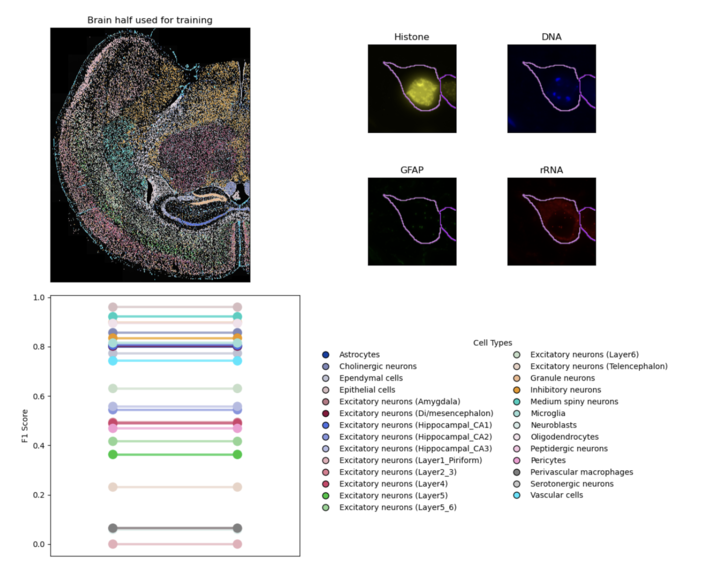
\includegraphics[width=.9\linewidth]{./figs/spatial.png}
\caption{\label{fig:spatial_omics}{[}PLACEHOLDER] Spatial omics analysis.}
\end{figure}
\section{Discussion}
\label{sec:org2b3c331}
The usage of image analysis pipelines that require manual setups hinders reproducibility and hinders our ability to compare different datasets. In this work we introduced our new library cp\_measure, which provides widely used engineered features and enables simpler automated analyses of microscopy data in either short scripts and complex pipelines. This also removes the requirement of using graphical interfaces to process microscopy data, resulting in better scaling capabilities for high-content microscopy data without the need of cloud-based infrastructure.

The biologically interpretable features provided by cp\_measure complement deep learning ones and offer a better mechanistic understanding of the underlying biology. When used in tandem with generalist tools it enables more insightful pipelines that leverage machine and deep learning approaches. 

These measurements have already been used in non-biological contexts, such as environmental monitoring \citep{ideharaExploringNileRed2025}, thus these engineered metrics also benefit other scientific fields beyond morphological profiling. In general, we see the decomposition of CellProfiler into modular components as a way to facili
\section{Future work}
\label{sec:org76eaf99}
There are multiple paths to improve and expand the functionality of cp\_measure. The first and most obvious is to integrate its measurements back to CellProfiler library. This would ensure that the results from pipelines built with either tool will be comparable in the future, while also providing the opportunity of formalizing the programmatic interface --- inputs and outputs --- of measurements.

Developing a comprehensive tests suite would guarantee mathematical correctness under the possible edge cases that may be encountered when dealing with new data. This test suite in turn would in turn open the door to further speed-ups in multiple ways: Firstly, optimizing the measurements that consume the most time, starting with object granularity (\textasciitilde{}80\% of the time). Additionally, it is possible to implement measurements using numba for just-in-time compiling and/or adding GPU support \citep{lamNumbaLLVMbasedPython2015}.

There is further space for improvement. First, provide a wrapper for all features that masp to scikit-image's regionprops as close as possible. Secondly, a list of essential measurements for use-cases where speed is more important than using all the features. By lowering the barrier of effort required to integrate cp\_measure into existing pipelines these 

Long-term, we envision cp\_measure can be the place to develop and distribute new measurements. While CellProfiler's measurements are widely used in bioimaging studies, the existing palette of measurements could be further extended to cover novel use-cases brought upon by novel developments in imaging acquisition devices and methods. Working with the community to further the number of measurements to better match the current questions scientists pose to imaging data.
\section{Methods}
\label{sec:orga949269}
\subsection{Data and software}
\label{sec:orgfc7bf0e}
The code for cp\_measure is available on \url{https://anonymous.4open.science/r/cp\_measure-B0DA}. All code to reproduce the analyses and figures, alongside links to the original data, is available on the Github repository \url{https://github.com/afermg/2025\_cpmeasure/}. The datasets we produced for this work are available on Zenodo, and the latest version can be found on \url{https://zenodo.org/records/15390631/latest}.

\bibliographystyle{icml2025}
\bibliography{bibliography,~/Documents/broad/bibliography/bibliography}
\end{document}
